
\section{Marco teórico}

\begin{frame}
\frametitle{Principal Components Analysis (PCA)}

\begin{itemize}
    \item Técnica de reducción de dimensionalidad que busca representar un conjunto de datos en un sistema de referencia de menos dimensiones mediante una combinación lineal de ''componentes principales''.
    \item Basa su principio en ubicar los datos de un conjunto en un nuevo sistema coordenado cuyos ejes (componentes principales) son ortogonales entre si y representan las variaciones más significativas entre los datos.
    \item Estos ejes pueden derivarse de diversas formas, como calcular la matriz de covarianza de los datos y obtener sus autovalores y autovectores respectivos.
\end{itemize}

\end{frame}

\begin{frame}
\frametitle{Principal Components Analysis (PCA)}

\begin{figure}
    \centering
    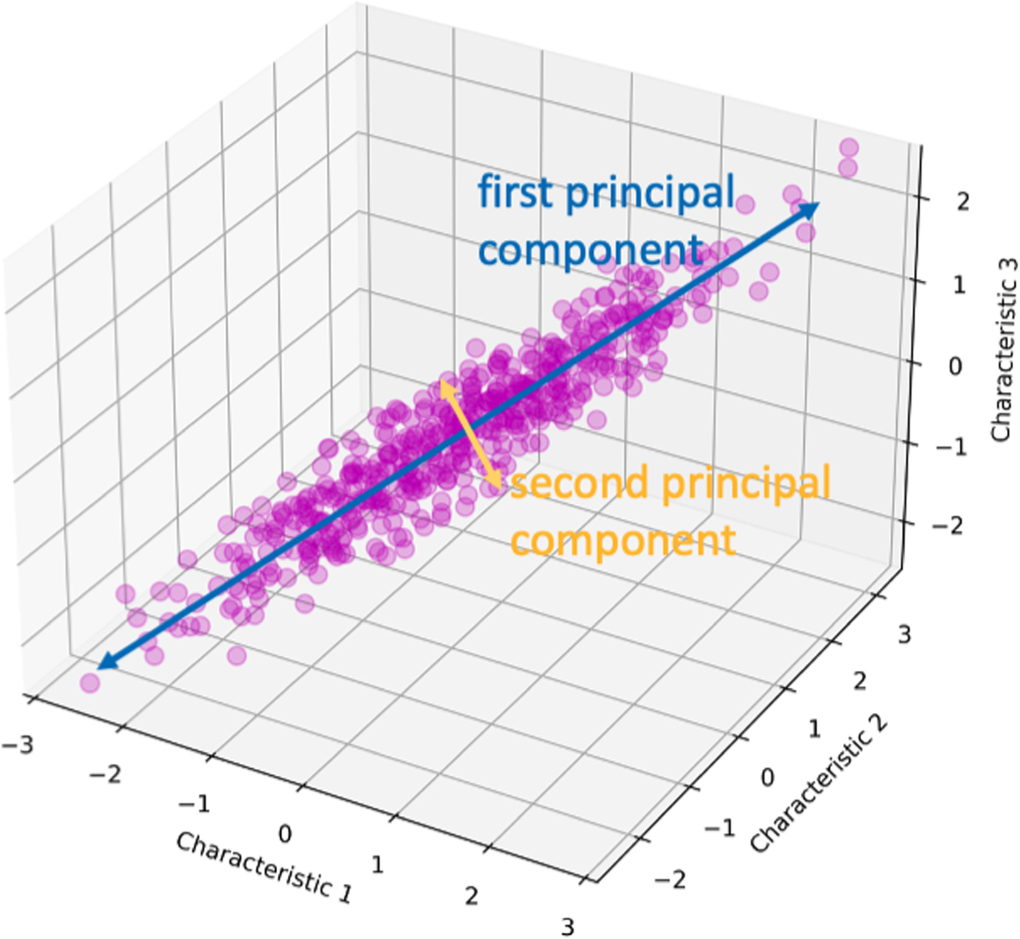
\includegraphics[width=0.35\linewidth]{images/pca.jpg}
    \caption{\footnotesize Ejemplo esquemático de PCA. Los datos originalmente se representan con 3 coordenadas ($x,y,z$). Sin embargo, uno podría representarlos de manera bien aproximada especificando una coordenada a través del vector que que describe la mayor variación en los datos (en azul). De añadirse más vectores de variación, con la condición de que sean ortogonales entre sí, puede representarse más precisamente la posición de cada punto. \citeblue{follette_introduction_2023}}
    \label{fig:pca}
\end{figure}

\end{frame}

\begin{frame}
\frametitle{Principal Components Analysis (PCA)}

\begin{itemize}
    \item La técnica de PCA, es ampliamente utilizada en el ámbito de detección de exoplanetas.
    \item Existe documentación de algoritmos que la utilizan para este objetivo, como \textit{Karhunen-Loève Image Processing} (KLIP) \citeblue{soummer_detection_2012}, a la vez que ya existen implementaciones accesibles en lenguajes de programación como \texttt{PynPoint} para Python \citeblue{amara_span_2012}.
\end{itemize}

\end{frame}

\begin{frame}
\frametitle{Principal Components Analysis (PCA)}

\begin{itemize}
    \item En particular, la librería \textit{Vortex Image Processing} (VIP) \citeblue{gomez_gonzalez_vip_2017}, implementada en Python, dispone de variadas herramientas para HCI, incluyendo un paquete de estimación de PCA basado en \texttt{PynPoint} y el trabajo de \textcolor{blue}{\cite{soummer_detection_2012}}.
\end{itemize}

\end{frame}

\begin{frame}
\frametitle{Angular Differential Imaging (ADI)}

\begin{itemize}
    \item La técnica de \textit{Angular Differential Imaging} (ADI) \citeblue{marois_angular_2006} aprovecha la rotación del cielo o \textit{Field of View} (FoV) para separar al ruido estático o cuasi-estático, propio del instrumento, de los cuerpos que se mueven.

    \item Se aplica calculando la mediana de todas las imágenes de un cubo de datos, sin embargo, VIP aplica una variación que utiliza la PCA de las imágenes en lugar de la mediana.
\end{itemize}


\end{frame}

\begin{frame}
\frametitle{Angular Differential Imaging (ADI)}
\begin{figure}
    \centering
    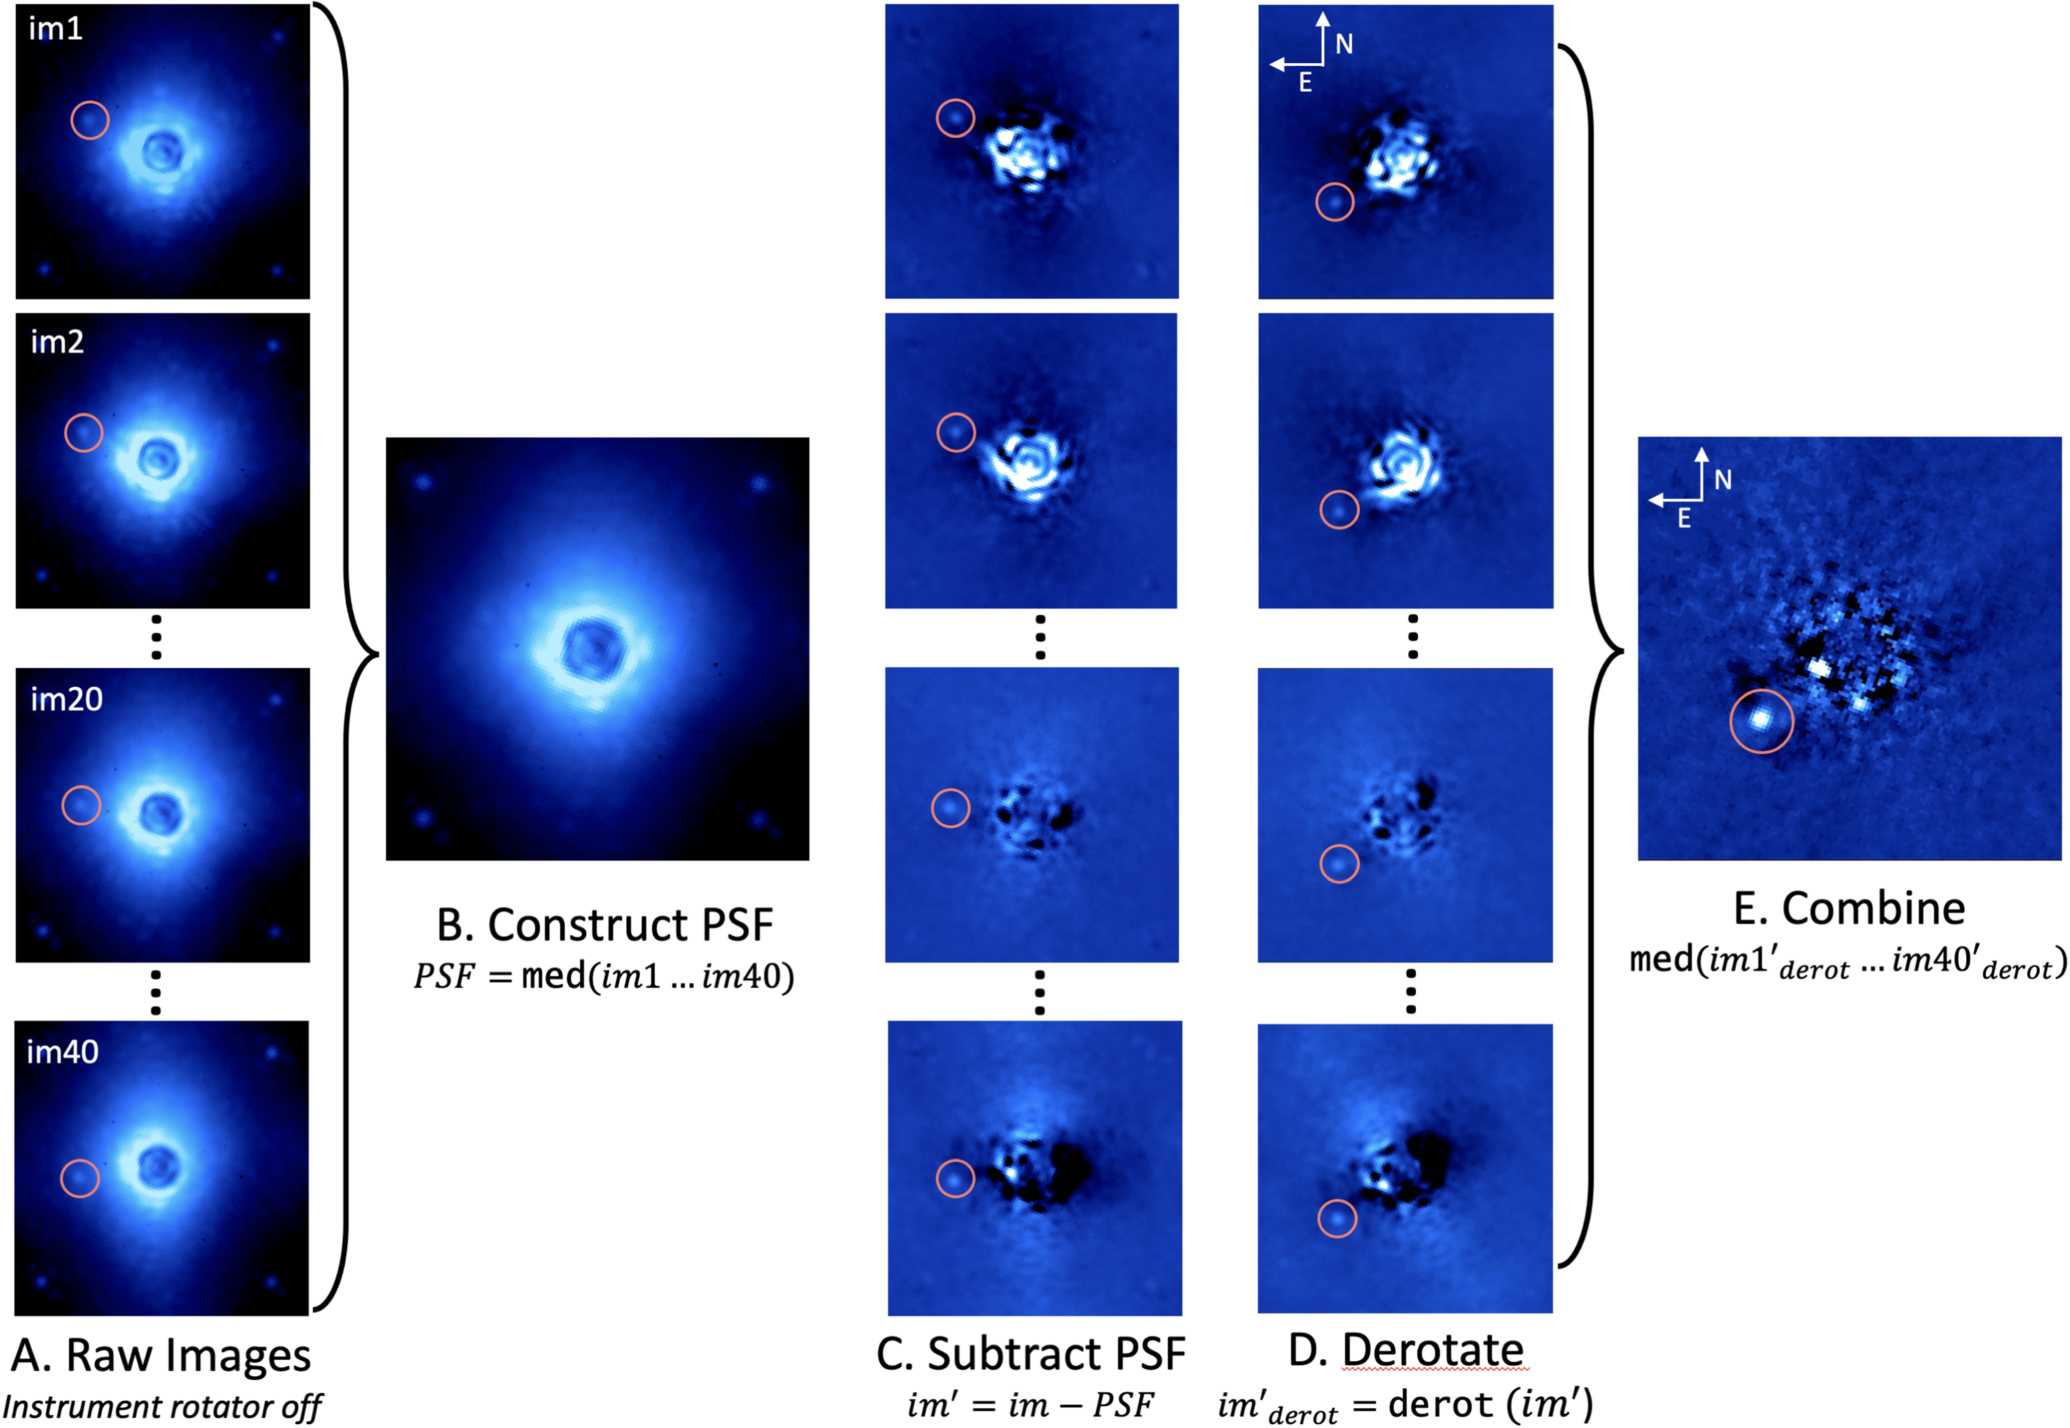
\includegraphics[width=0.7\linewidth]{images/adi.jpg}
    \caption{Ejemplo de detección de un exoplaneta utilizado ADI con la mediana. \citeblue{follette_introduction_2023}}
    \label{fig:adi}
\end{figure}

\end{frame}

\begin{frame}
\frametitle{Angular Differential Imaging (ADI)}
\begin{figure}
    \centering
    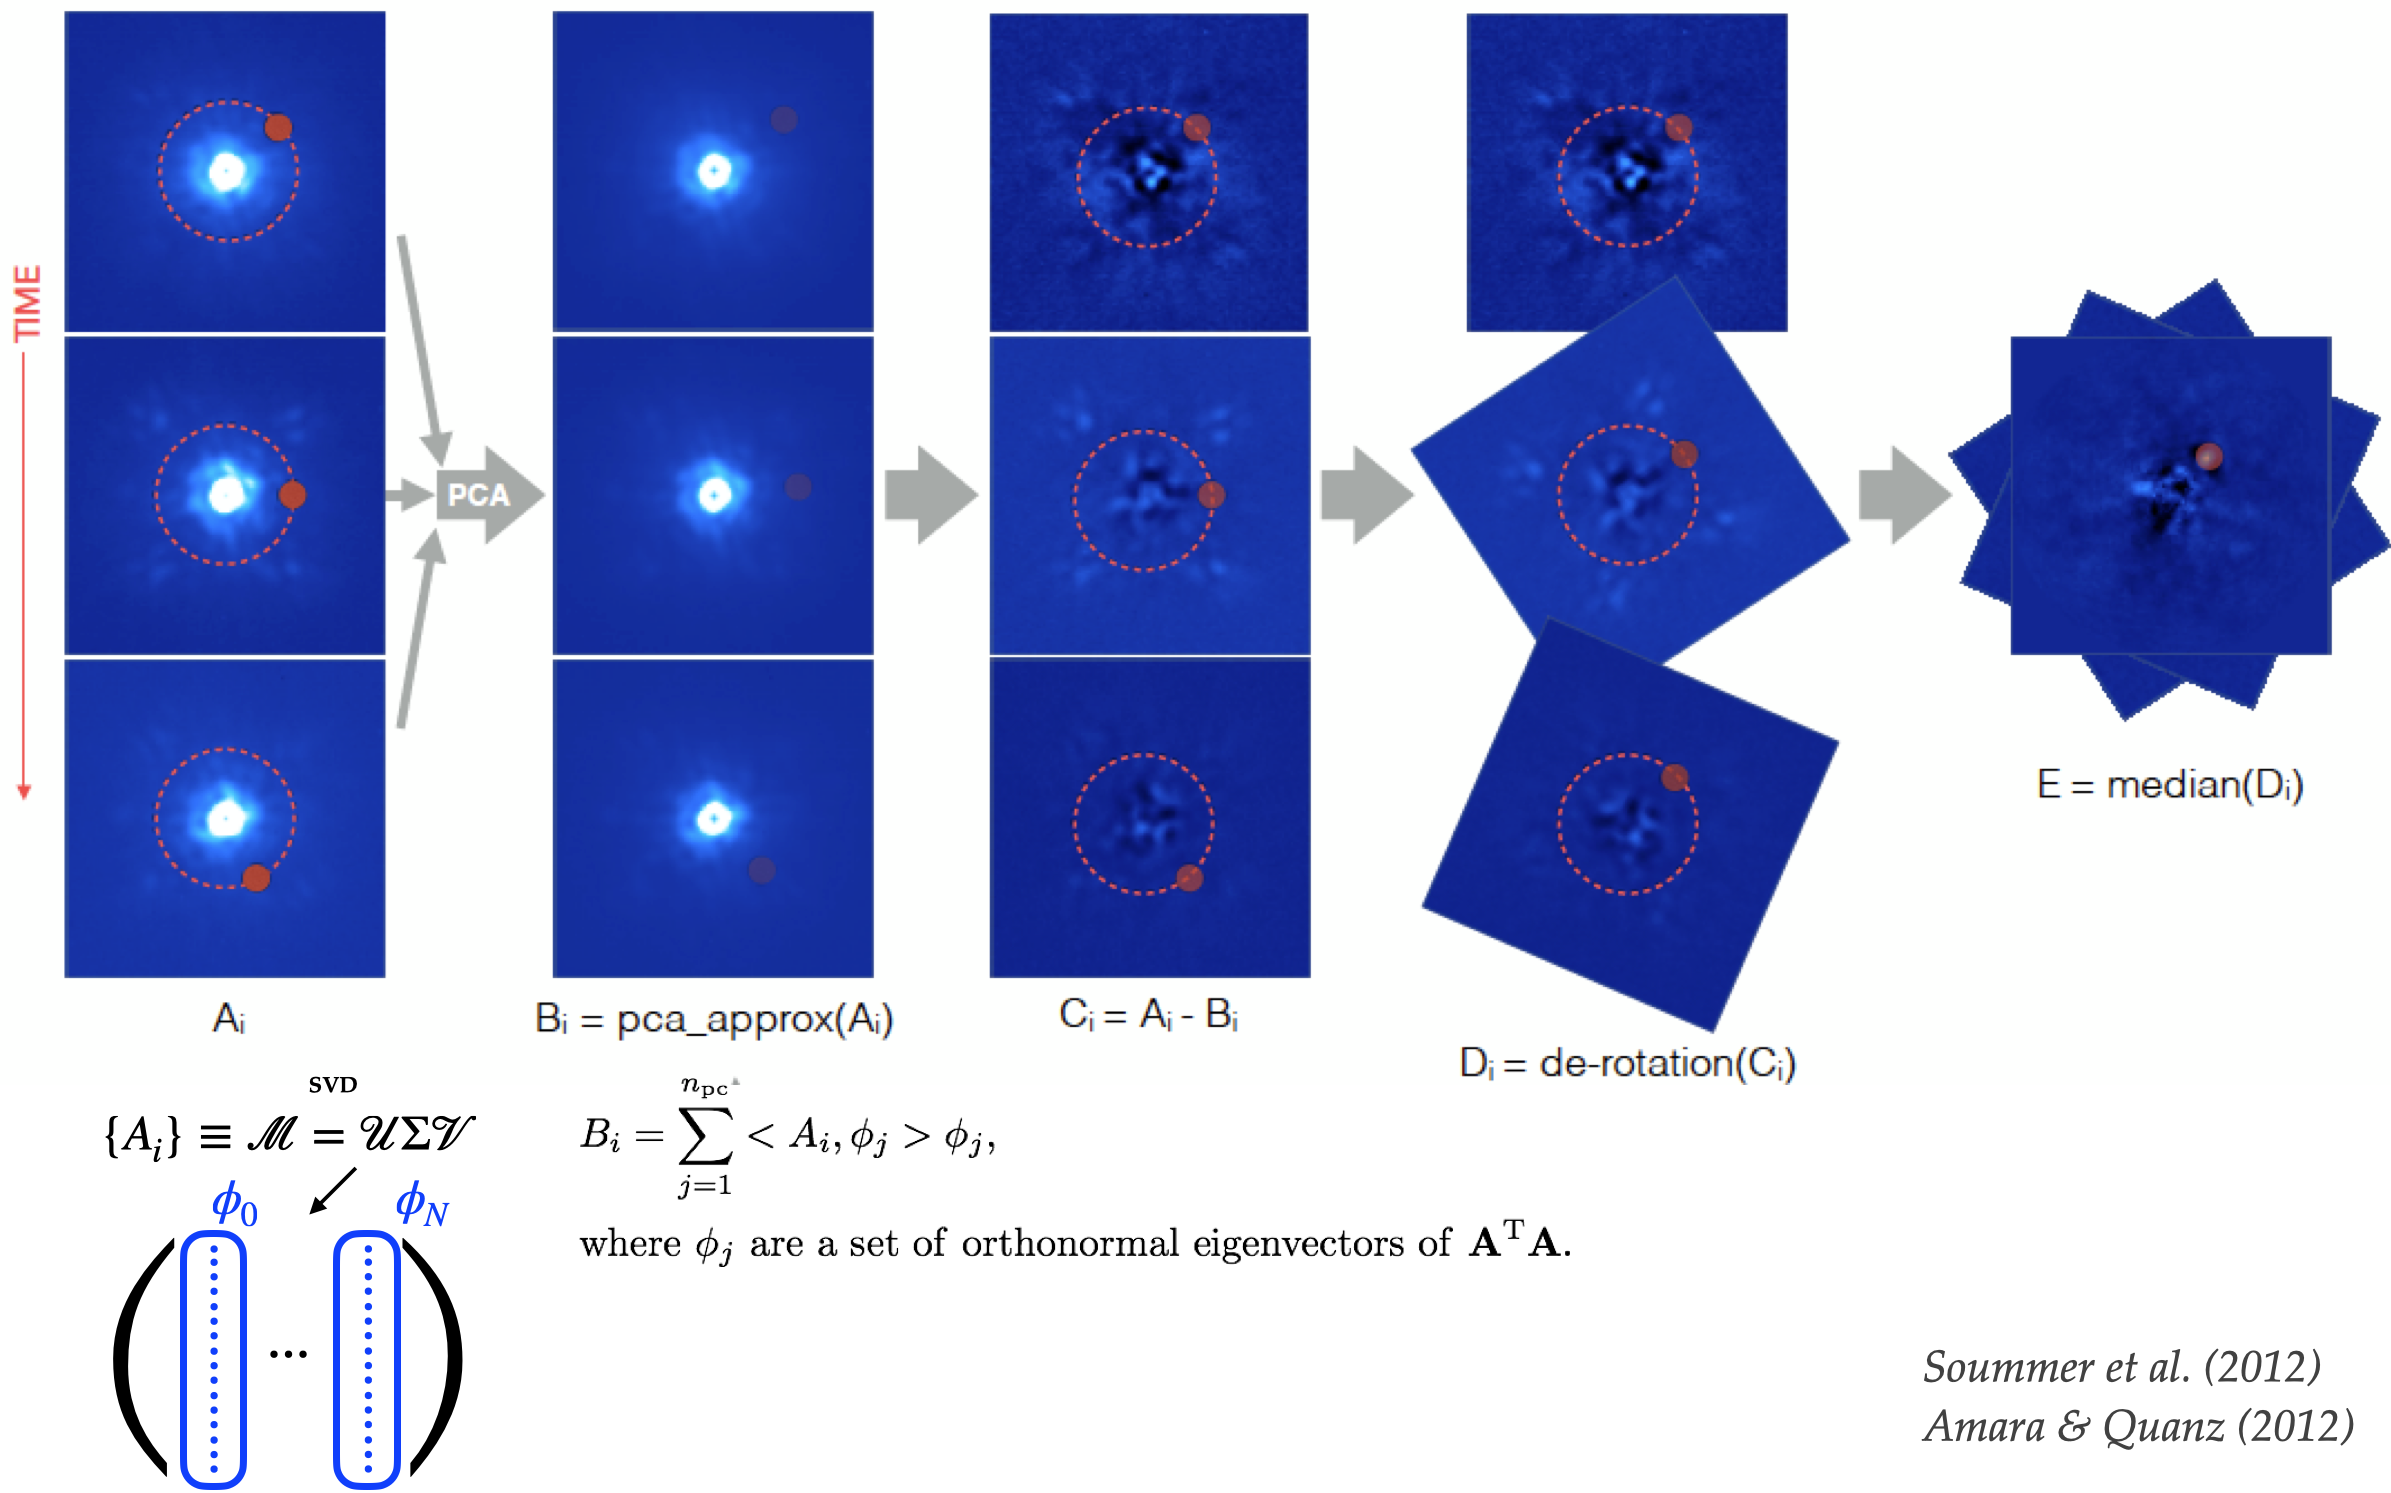
\includegraphics[width=0.7\linewidth]{images/adi_pca.png}
    \caption{Ejemplo de detección de un exoplaneta utilizado ADI con PCA. Fuente: \textcolor{magenta}{\href{https://vip.readthedocs.io/en/v1.4.0/tutorials/03_psfsub.html\#3.5.1.-Full-frame-PCA}{VIP}}}.
    \label{fig:adi_pca}
\end{figure}

\end{frame}

%---------------------------------------------------------

